% !TeX document-id = {31cec06c-209e-42c6-b48d-393b1a0af1d2}
% !TeX TS-program = xelatex
% !BIB TS-program = biber
% !TeX encoding = UTF-8
% !TeX spellcheck = en_US
% !TeX root = seminar_presentation__intelligent_industrial_robots.tex


%% LaTeX-Beamer template for KIT design
%% by Erik Burger, Christian Hammer
%% title picture by Klaus Krogmann
%%
%% version 2.1
%%
%% mostly compatible to KIT corporate design v2.0
%% http://intranet.kit.edu/gestaltungsrichtlinien.php
%%
%% Problems, bugs and comments to
%% burger@kit.edu

\documentclass[18pt]{beamer}

\usepackage[utf8]{inputenc}

%% SLIDE FORMAT

% use 'beamerthemekit' for standard 4:3 ratio
% for widescreen slides (16:9), use 'beamerthemekitwide'
% for widescreen slide without sidebar use 'beamerthemekitwidenosidebar'

%\usepackage{templates/beamerthemekit}
%\usepackage{templates/beamerthemekitwide}
\usepackage{templates/beamerthemekitwidenosidebar}

% use this to disable the latex beamer navigation symbols
%\beamertemplatenavigationsymbolsempty


%% TITLE PICTURE

% if a custom picture is to be used on the title page, copy it into the 'logos'
% directory, in the line below, replace 'mypicture' with the 
% filename (without extension) and uncomment the following line
% (picture proportions: 63 : 20 for standard, 169 : 40 for wide
% *.eps format if you use latex+dvips+ps2pdf, 
% *.jpg/*.png/*.pdf if you use pdflatex)

\titleimage{plc_logo}

%% TITLE LOGO

% for a custom logo on the front page, copy your file into the 'logos'
% directory, insert the filename in the line below and uncomment it

\titlelogo{iar_iirob}

% (*.eps format if you use latex+dvips+ps2pdf,
% *.jpg/*.png/*.pdf if you use pdflatex)

%% TikZ INTEGRATION

% use these packages for PCM symbols and UML classes
\usepackage{templates/tikzkit}
\usepackage{templates/tikzuml}

\usepackage{tabularx}
\usepackage{multirow}
\usepackage{multicol}
\usepackage{booktabs}

\usepackage{glossaries}
\usepackage{acronym}
\usepackage{listings}

% the presentation starts here

\title[Automated Programming of Programmable Logic Controllers]{Seminar Intelligent Industrial Robots}
\subtitle{Automated Programming of Programmable Logic Controllers}
\author{David Oberacker}

\institute{
	Institute for Anthropomatics and Robotics - Intelligent Process Automation and Robotics Lab (IAR-IPR)
}

% Bibliography

\usepackage[citestyle=authoryear,bibstyle=numeric,hyperref,backend=biber]{biblatex}
\addbibresource{presentation.bib}
\bibhang1em

\newacronym{acn:PLC}{PLC}{Programmable Logic Controller}
\newacronym{acn:UML}{UML}{Unified Modeling Language}
\newacronym{acn:SysML}{SysML}{Systems Modeling Language}

\makeglossaries

\begin{document}

% change the following line to "ngerman" for German style date and logos
\selectlanguage{english}

%title page
\begin{frame}
\titlepage
\end{frame}

%\begin{frame}{Introduction}
%    \begin{figure}
%        \centering
%        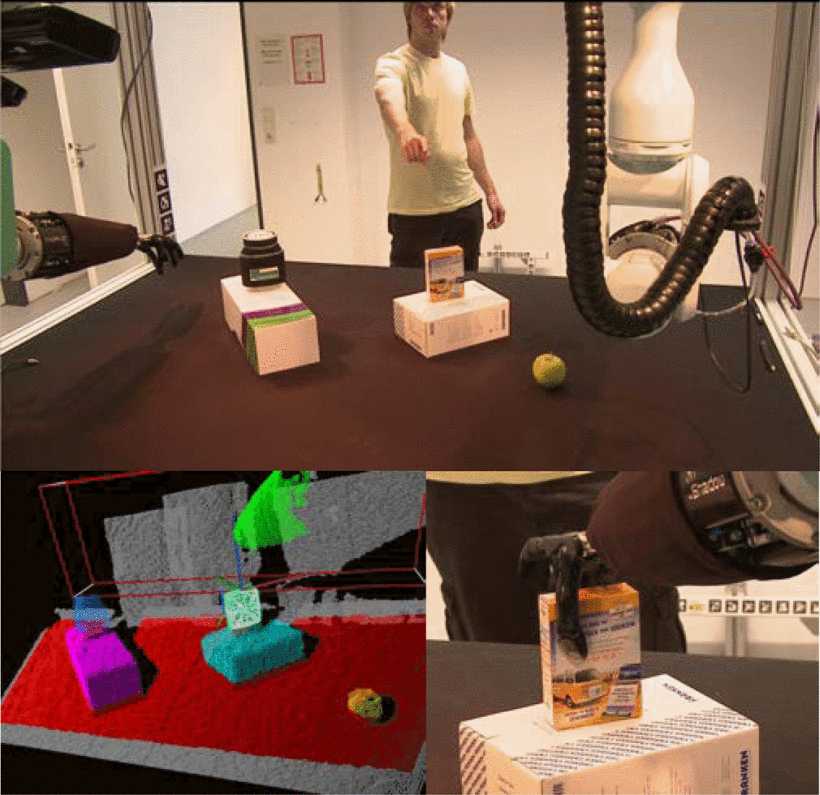
\includegraphics[height=0.7\textheight]{figures/3d_semantic_grasping.png}
%    \end{figure}
%\footcitetext{6385692}
%\end{frame}

%table of contents
%\begin{frame}{Outline}
%\tableofcontents
%\end{frame}

\section{Introduction}

\begin{frame}{Introduction}
    
    \begin{itemize}
        \item Automation is an important factor.
        \item Industry 4.0 requires flexibility.
        \item \acrfull{acn:PLC} are common.
        \item Programming of~\acrshort{acn:PLC} is non-flexible.
    \end{itemize}
    \pause
    $\Rightarrow $ Are there ways to program a~\acrshort{acn:PLC} in a more flexible way ?
    
\end{frame}

\section{Programmable logic controller}

\begin{frame}{Programmable Logic Controller}
\begin{columns}
    \begin{column}{0.5\textwidth}
        \begin{itemize}
            \item Specialized industrial computers.
            \item \textbf{Cycle based} execution semantic:
            \begin{enumerate}
                \item Read~\textbf{input} values.
                \item \textbf{Execute} the~\textbf{user program}.
                \item Publish~\textbf{output} values.
            \end{enumerate}
            \item Standardized IEC 61131-3 programming languages.
        \end{itemize}
    \end{column}
    \begin{column}{0.5\textwidth}
        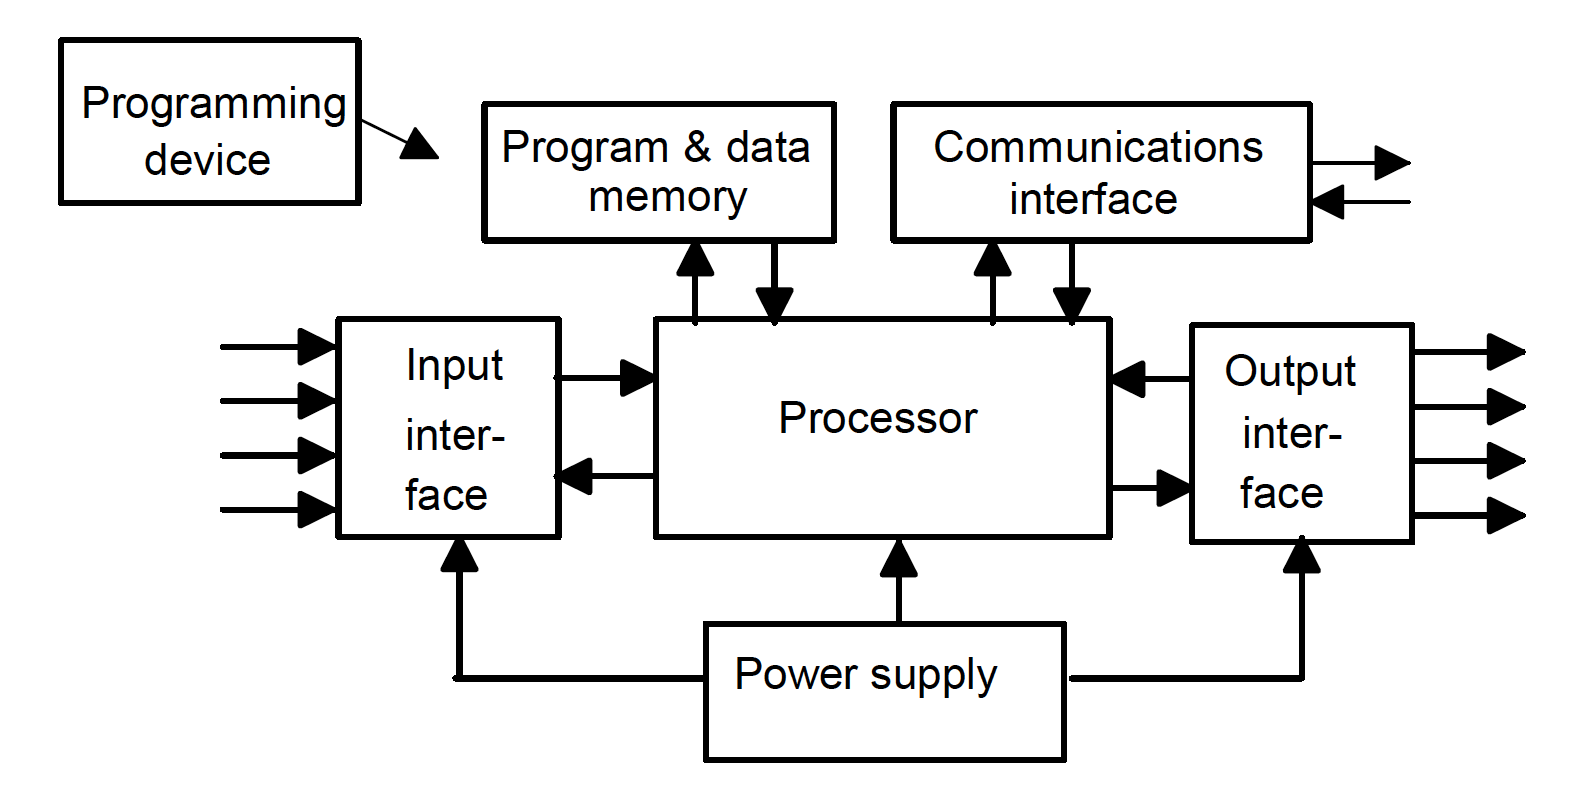
\includegraphics[width=\textwidth]{figures/PLC_Architecture.png}
        {\footnotesize Source:~\cite{BOLTON200653}}
    \end{column}
\end{columns}
\end{frame}

\subsection{IEC 61131-3 Languages}

\begin{frame}{IEC 61131-3 Languages}
    \begin{columns}
    	\begin{column}{0.5\textwidth}
    		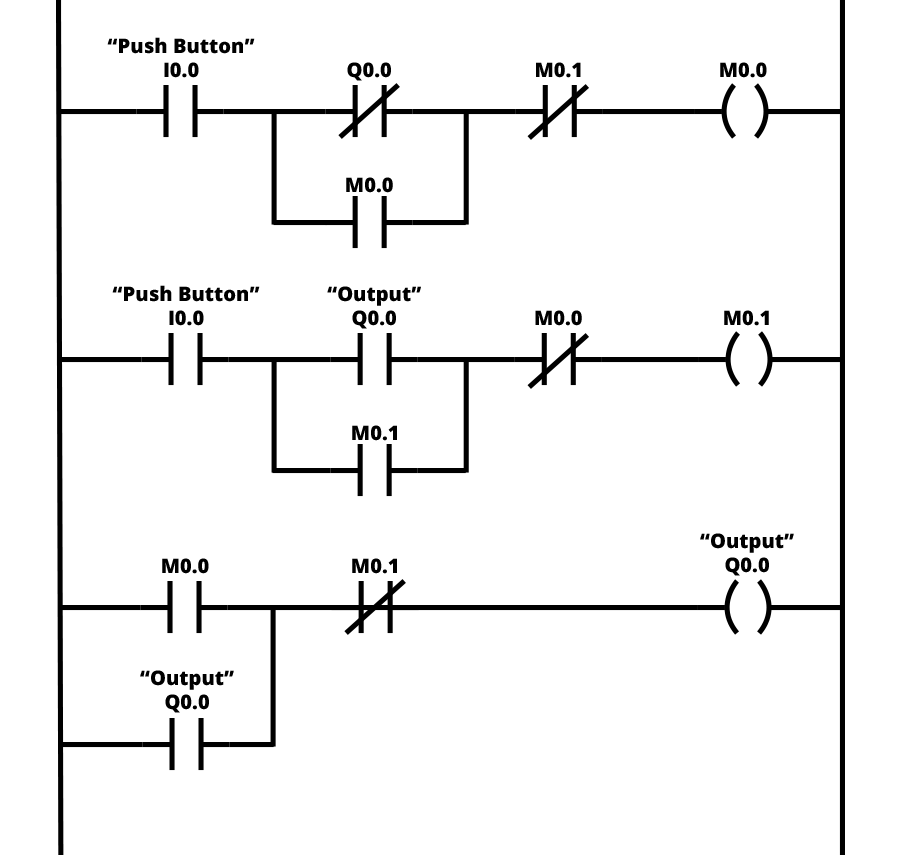
\includegraphics[width=0.8\textwidth]{figures/ld.png}
           {\footnotesize  Source:~\url{https://www.plcacademy.com/ladder-logic-examples/}}
    	\end{column}
        \begin{column}{0.5\textwidth}
            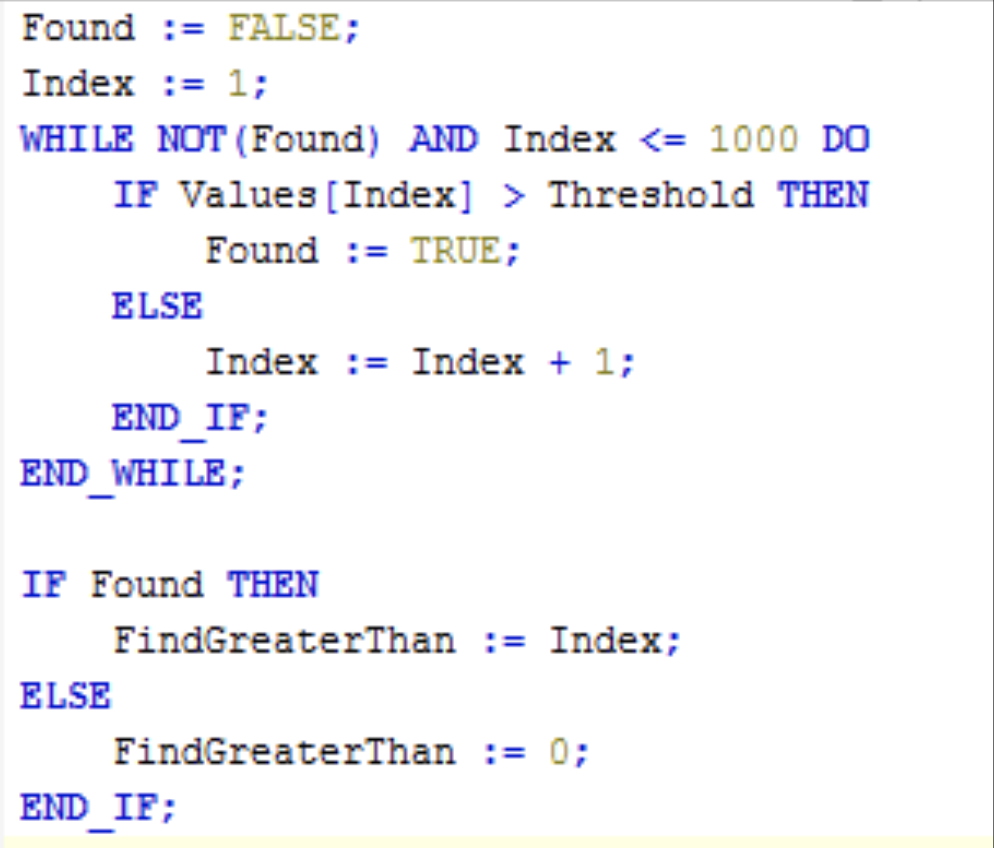
\includegraphics[width=0.8\textwidth]{./figures/st.png}
            {\footnotesize Source:~\url{http://www.contactandcoil.com/twincat-3-tutorial/structured-text/}}
        \end{column}
    \end{columns}
\end{frame}

\section{Automated programming of PLCs}

\begin{frame}{Automated programming of PLCs}
    \begin{itemize}
        \item The IEC 61131-3 languages are procedural.
        \item Not optimized for larger or dynamic systems.
        \item No support for modern software engineering methods.
        \begin{itemize}
            \item Rapid changes to the system.
            \item Validation and verification.
        \end{itemize}
    \end{itemize}
    $\Rightarrow$ Possible Solution:~\textbf{Automated generation} of IEC 61131-3 code.
\end{frame}

\subsection{C/C++-based programming}

\begin{frame}{C/C++-based programming}
\begin{itemize}
	\item Widespread systems programming languages.
    \item They support high-level abstractions (e.g. classes, modules).
    \item Supported by two~\acrshort{acn:PLC} development environments:
    \begin{itemize}
        \item Beckhoff TwinCAT3 
        \item B\&R Automation Studio
    \end{itemize}
\end{itemize}
\pause
$\Rightarrow$ High-level programming is supported; Automatic generation of code or validation is not supported.
\end{frame}

\subsection{Formal description based}

\begin{frame}{Formal specification based}
\begin{itemize}
    \item Code generation from a formal specification.
    \item Design from a high-level abstraction.
    \item Widespread practice in software engineering.
\end{itemize}
In the following section I present these formalizations:
\begin{itemize}
    \item UML/SysML
    \item Simulink
    \item PLCspecif
\end{itemize}
\end{frame}

\begin{frame}{UML / SysML}
\begin{columns}
    \begin{column}{0.6\textwidth}
        \begin{itemize}
            \item \acrfull{acn:UML}
            \item  \acrfull{acn:SysML}
            \item Behavior: state-charts.
            \item Structure: class-diagrams..
            \item \cite{WITSCH2015} and~\cite{VH:2014} define plcML
            \begin{itemize}
                \item Faster and more reliable development.
                \item Model can be translated into ST code.
            \end{itemize}
        \end{itemize}
    \end{column}
    \begin{column}{0.4\textwidth}
        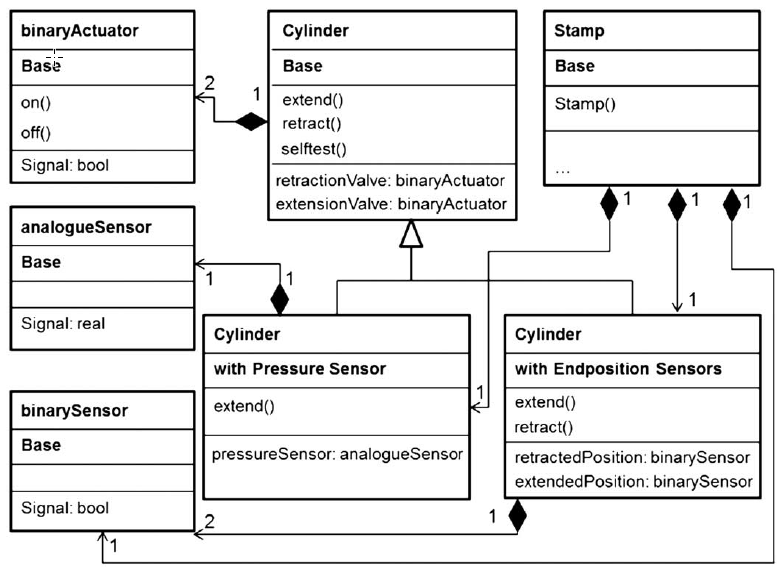
\includegraphics[width=\textwidth]{./figures/modAT4rMS_struct.png}
       {\footnotesize  Source:~\cite{VH:2014}}
    \end{column}
\end{columns}

\end{frame}

\begin{frame}{Simulink}
\begin{columns}
    \begin{column}{0.5\textwidth}
        \begin{itemize}
            \item Modeling software for the MATLAB environment.
            \item Model, Simulate \& Verify.
            \item Supports translation to ST.
            \item Easy to use method.
            \item Scales well.
        \end{itemize}
    \end{column}
    \begin{column}{0.5\textwidth}
        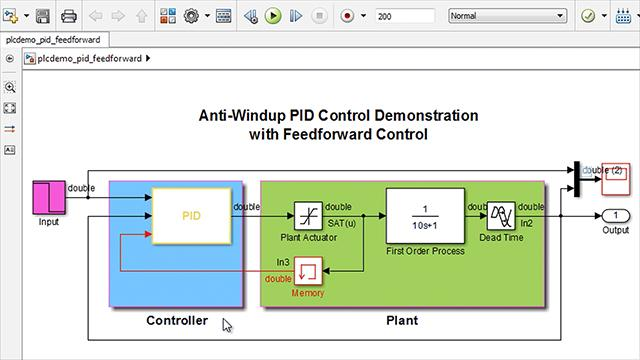
\includegraphics[width=\textwidth]{./figures/simulink.jpg}
       {\footnotesize  Source:~\url{https://de.mathworks.com/videos/simulink-plc-coder-overview-61206.html}}
    \end{column}
\end{columns}
\end{frame}

\begin{frame}{plcSpecif}
    \begin{itemize}
        \item Developed by \cite{7819191}.
        \item Module based specification.
        \item Verification methods are presented.
        \item Focus on ease of use \& traceability.
        \item Reliability as a core feature.
    \end{itemize}
\end{frame}

\section{Risks of automated programming}

\begin{frame}{Risks of automated programming}
\begin{itemize}
    \item Safety and real-time use cases.
    \item Clear assessment of possible risks required.
    \item Inherent risks to code generation.
\end{itemize}
$\Rightarrow$ They need to be addressed before the system can be deployed!
\pause
\\
Two components of the risk are addressed:
\begin{itemize}
    \item Transformation function correctness
    \item Runtime behavior guarantees
\end{itemize}
\end{frame}

\begin{frame}{Risks of automated programming}

\begin{block}{Transformation function correctness}
	\begin{itemize}
		\item Consistency between the code and modeled behavior.
        \item Often no detailed analysis.
        \item Traceability should be possible.
	\end{itemize}
\end{block}
\pause
\begin{block}{Runtime guarantees}
    \begin{itemize}
        \item Runtime behavior is the relevant factor.
        \item Custom state machines that work over multiple PLC cycles.
        \item Verification on the target platform.
    \end{itemize}
\end{block}
\end{frame}

\section{Conclusions}
\begin{frame}{Conclusions}

\begin{itemize}
    \item New programming methods are required.
    \pause
    \item Automated code generation is a viable options.
    \pause
    \item Well supported and capable approaches available 
    \begin{itemize}
        \item Simulink PLC coder
        \item plcML
    \end{itemize}
    \pause
    \item Effecitve and efficient.
    \pause
    \item High user acceptance and lower initial skill requirements.
    \pause
    \item Efficient methods for risk analysis and verification are required.
\end{itemize}
\end{frame}

\begin{frame}
\vfill
\centering
{\LARGE Thank you for your attention.}\\
\vspace{1cm}
{\Large \textbf{Questions ?}}
\vfill
\end{frame}

\appendix
\beginbackup

\begin{frame}[allowframebreaks]{Glossaries}
\printglossaries
\end{frame}

\begin{frame}[allowframebreaks]{References}
\printbibliography
\end{frame}

\backupend

\end{document}
\grid
